\section{An\'alisis y Resultados}

    \subsection{Valor de RTO variando $\alpha$ y $\beta$}

        Primero estudiamos como var\'ia el \rto{} cuando se utilizan los
        valores extremos de $\alpha$ y $\beta$. Se utiliz\'o un valor
        de delay = \textit{6 ticks} sin probabilidad de p\'erdida.

        Puede verse en la \textit{Figura 1}, que tomando $\alpha=0$,
        $\beta=0$ los cálculos ignoran por completo los nuevos
        valores de RTT y consideran únicamente los valores de SRTT
        anteriores. En este caso, el valor constante inicial.

        La \textit{Figura 2} muestra como al tomar ambas variables el valor
        1, los cálculos ignoran los valores anteriores (tanto de variación
        de RTT (RTTVAR) como de SRTT), y modifican los resultados
        únicamente en función de la última muestra de RTT obtenida. El
        resultado es un gráfico en donde el RTO coincide exactamente con
        el SRTT, y ambos responden excesivamente a cualquier fluctuación
        que se produzca en el valor del RTT.

        Por otra parte, la \textit{Figura 3} muestra lo que sucede al
        ponderar de igual manera los valores anteriores con los nuevos, al
        tomar ambas variables con valor 0.5. Esto debería generar valores
        cercanos a los de las muestras anteriores, pero que sean capaces
        de responder a cambios significativos y permanentes del valor de
        RTT. En otras palabras, que alcancen un equilibrio entre ambas
        propuestas. Sin embargo, el comportamiento no fue el esperado.

        El resultado es una serie de cálculos demasiado sensibles a las
        fluctuaciones temporales que responden excesivamente a estos
        cambios. Por ello hicimos una \'ultima prueba (\textit{Figura 4})
        donde fijamos el valor de $\alpha$ en 0.15 y $\beta$ en 0.20
        (cercanos al propuesto por el RFC 6298).
        Las conexiones en las distintas redes por lo general permanecen
        estables la mayor parte del tiempo, por lo que los cambios bruscos
        de \rtt{} son poco probables. Por otro lado el valor de $\beta$
        permite agregar un poco de sensibilidad a los cambios en el valor
        de los \textit{rtts}.

        \begin{figure}[H]
	    \center
	    \begin{subfigure}{0.48\textwidth}
		    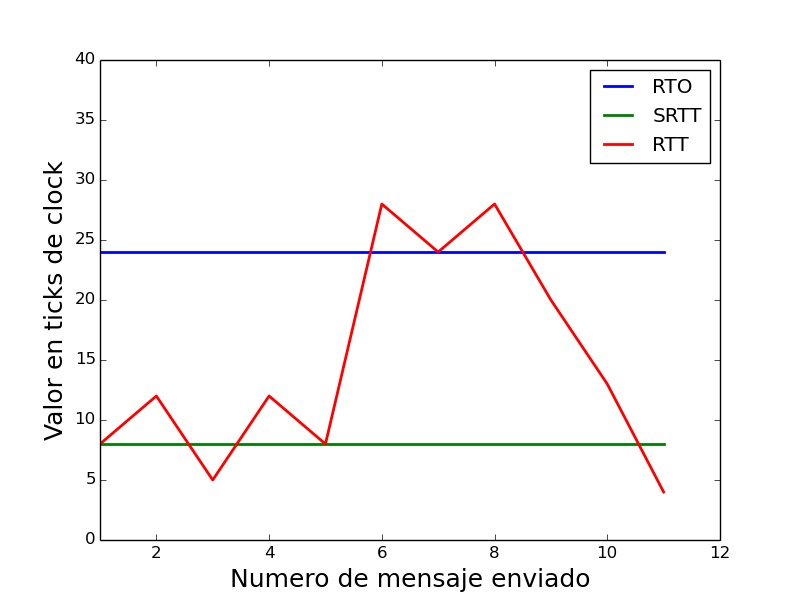
\includegraphics[width=1.0\textwidth]{imagenes/test_0_0.jpg}
		    \caption*{Figura 1}
	    \end{subfigure}
	    ~
	    \begin{subfigure}{0.48\textwidth}
		    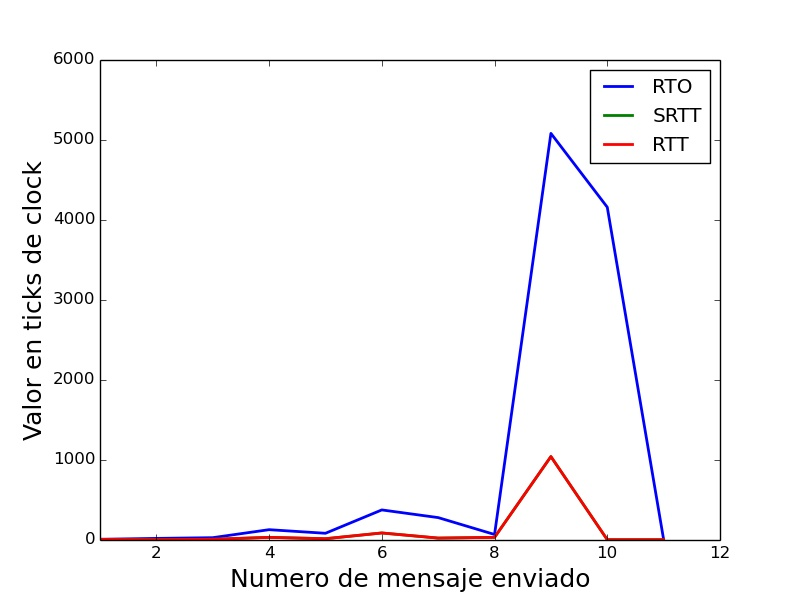
\includegraphics[width=1.0\textwidth]{imagenes/test_1_1.jpg}
		    \caption*{Figura 2}
	    \end{subfigure}
	    \end{figure}

        \begin{figure}[H]
	    \center
	    \begin{subfigure}{0.48\textwidth}
		    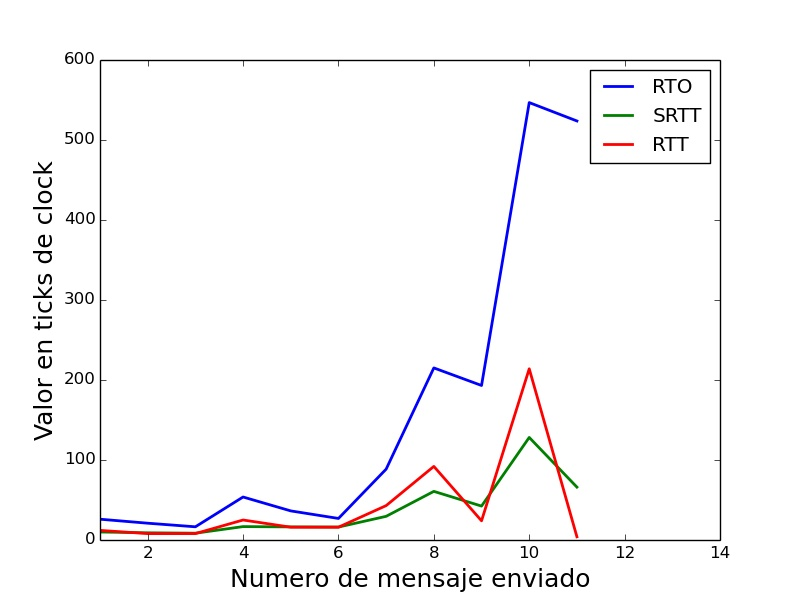
\includegraphics[width=1.0\textwidth]{imagenes/test_5_5.jpg}
		    \caption*{Figura 3}
	    \end{subfigure}
	    ~
	    \begin{subfigure}{0.48\textwidth}
		    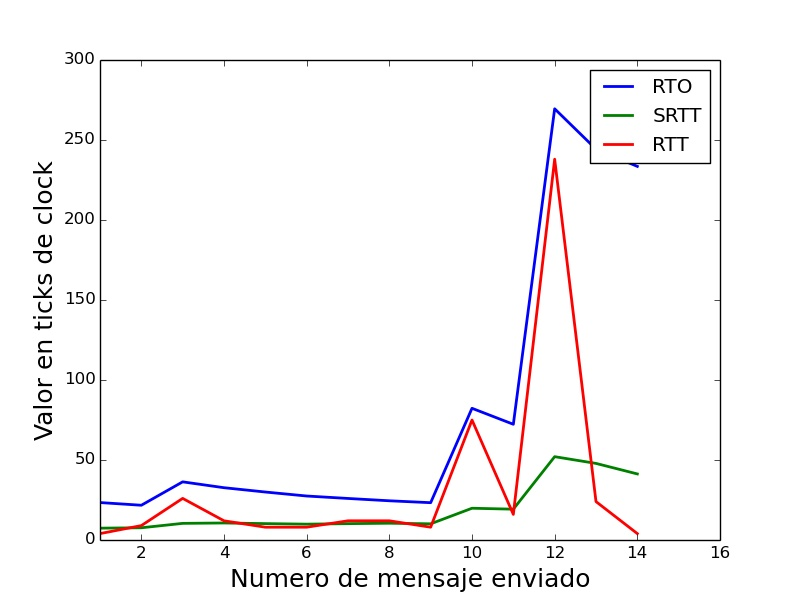
\includegraphics[width=1.0\textwidth]{imagenes/test_a_b.jpg}
		    \caption*{Figura 4}
	    \end{subfigure}
	    \end{figure}

        Finalmente intentamos medir muchos valores de \rto{} para
        diversas convinaciones de $\alpha$ y $\beta$.
        Los resultados de medir el \rto{} para un valor fijo de
        \textit{25 ticks} y probabilidad de perdida cero luego de
        enviar 200 paquetes se pueden ver en la \emph{Figura 4}.

    \subsection{Perdida de paquetes variando $\alpha$ y $\beta$}
        Para estudiar la perdida de paquetes se fij\'o el valor de
        de \rto{} en \textit{25 ticks} y no se simularon p\'erdidas.
        Sin embargo en varios casos hubo retransmisiones, la 
        \textit{Figura 5} muestra la cantidad que hubo durante el env\'io de 300
		paquetes.        
    \begin{figure}[H]
	    \center
	    \begin{subfigure}{0.45\textwidth}
		    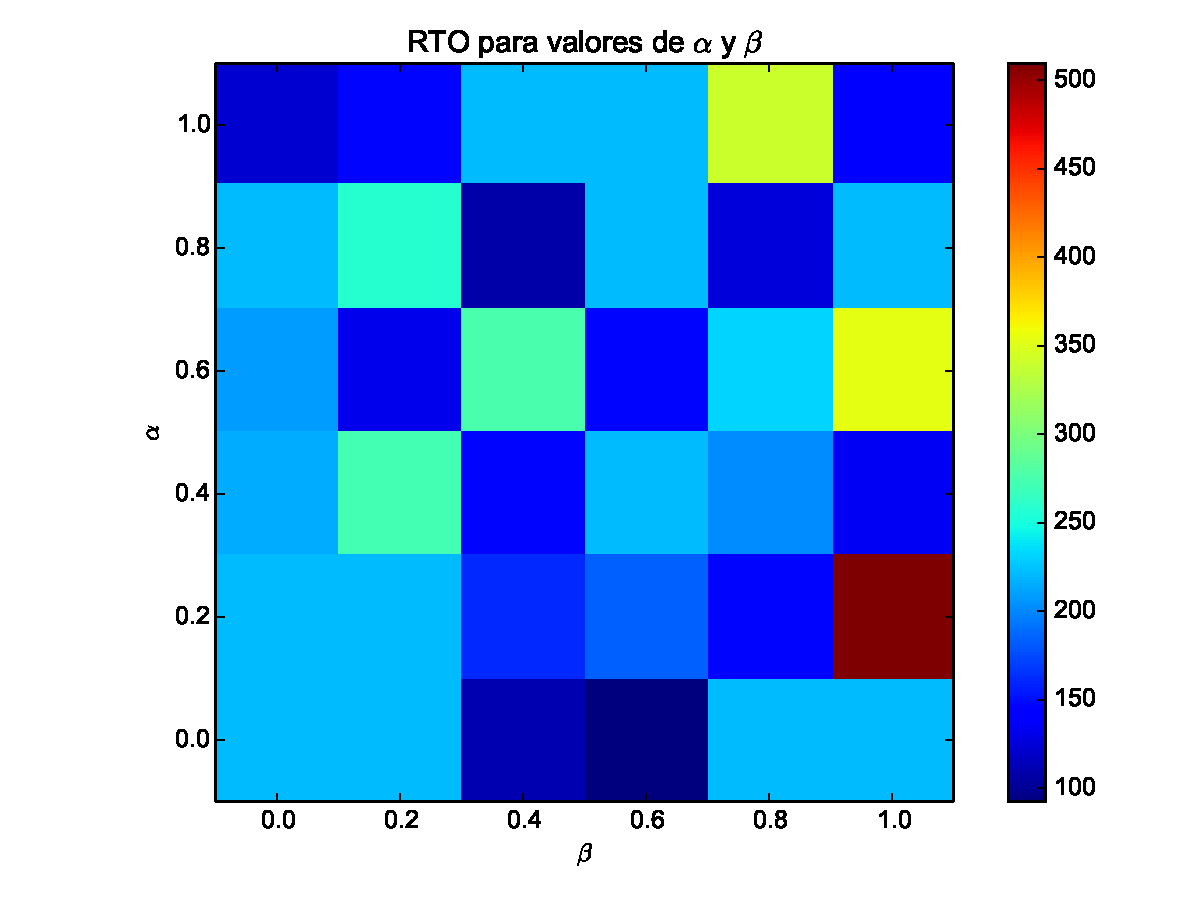
\includegraphics[width=1.0\textwidth]{imagenes/rto_vs_alphaBeta.pdf}
		    \caption*{Figura 4}
	    \end{subfigure}
	    ~
	    \begin{subfigure}{0.45\textwidth}
		    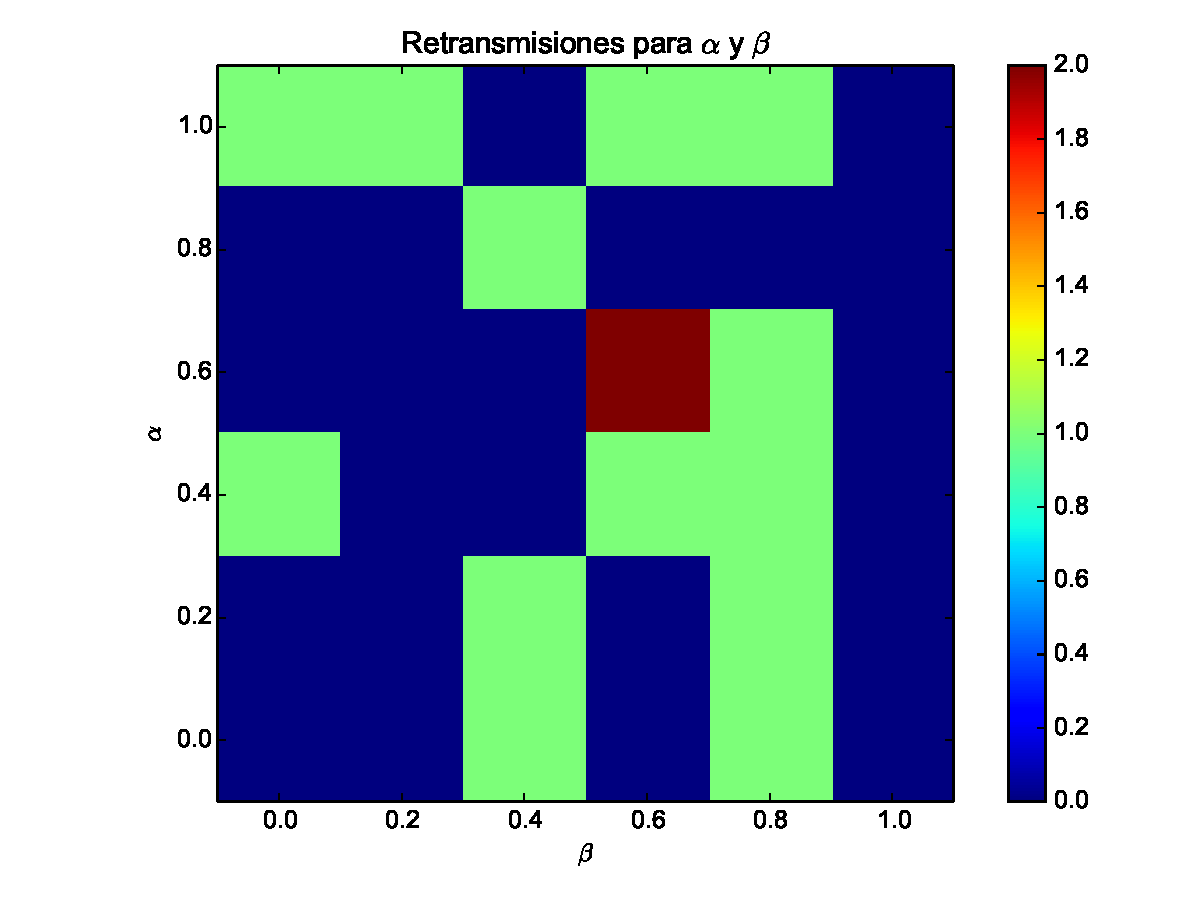
\includegraphics[width=1.0\textwidth]{imagenes/retransmisiones_300.pdf}
		    \caption*{Figura 5}
	    \end{subfigure}
    \end{figure}

	Seg\'un una interpretaci\'on de estos heatmaps dice que $\alpha$ y $\beta$
	no tienen una relaci\'on directae en el valor de RTO, pero que los valores
	m\'as bajos vienen cuando $\alpha$ es lo m\'as chico posible y $\beta$
	cercano a $0.6$, o cuando $\alpha$ es lo m\'as grande posible y $\beta$ lo
	m\'as chico posible.

	Con el segundo, vemos que tampoco hay una relaci\'on directa entre los
	valores y $\alpha$ o $\beta$ que nos permita hacer una decisi\'on simple
	sobre el mejor elemento de estos valores. Sin embargo, podemos ver que
	asignando 1.0 a $\beta$, las retransmisiones siempre son m\'imimas.

	\newpage
    \subsection{Valor de RTO cuando la red se congestiona sin perdida}
        Para este configuramos el cliente para que env\'ie 600 paquetes al
        servidor, pero luego de enviarse 300 paquetes, el delay de la red
        se duplicara o cuadruplicara.

        El \emph{Escenario 1} muestra el resultado en una red con
        par\'aemtros: $\alpha={{1}\over{2}}$, $\beta={{1}\over{4}}$
        cuando no se congestiona, cuando la congesti\'on causa el doble de
        delay, y cuando causa el cu\'adruple.

        \begin{figure}[H]
            \center

		    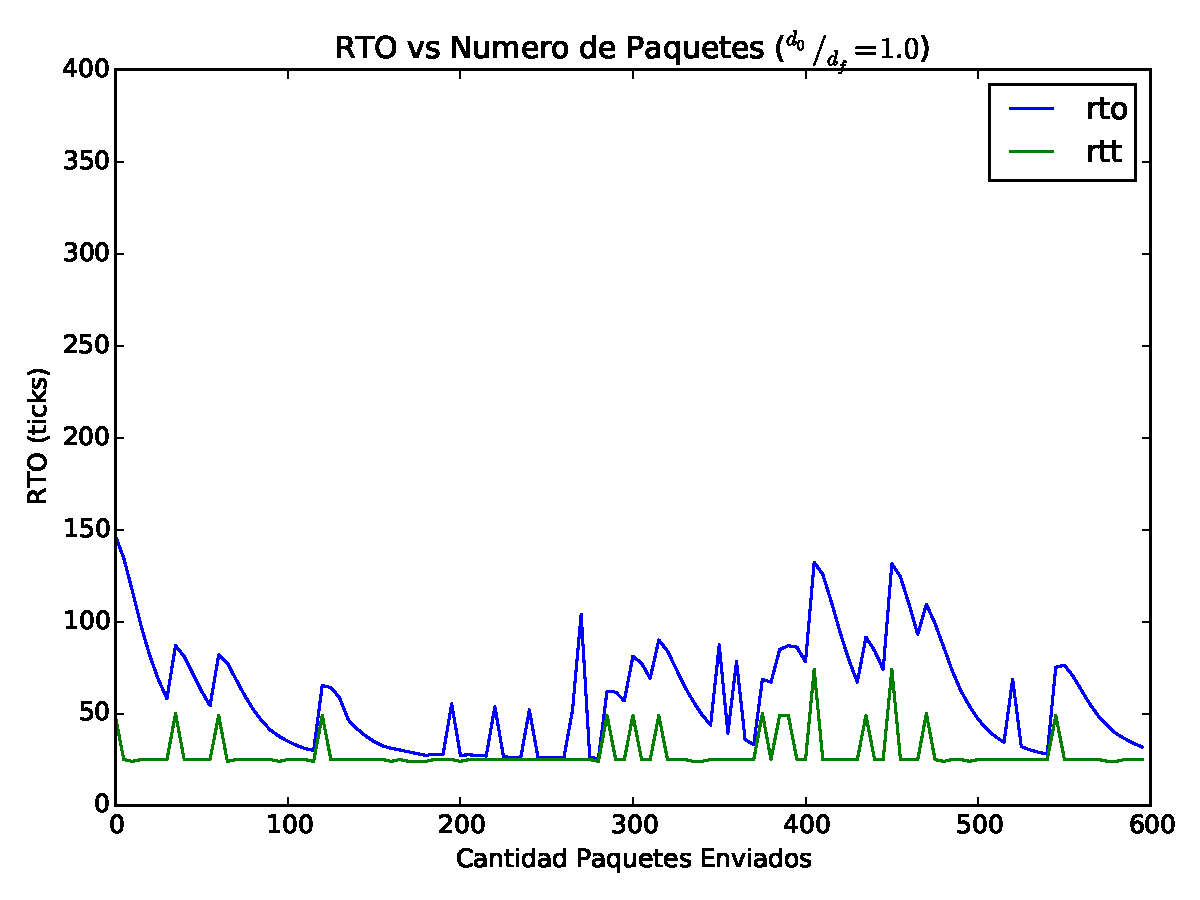
\includegraphics[width=0.32\textwidth]{imagenes/congestion_1.pdf}
		    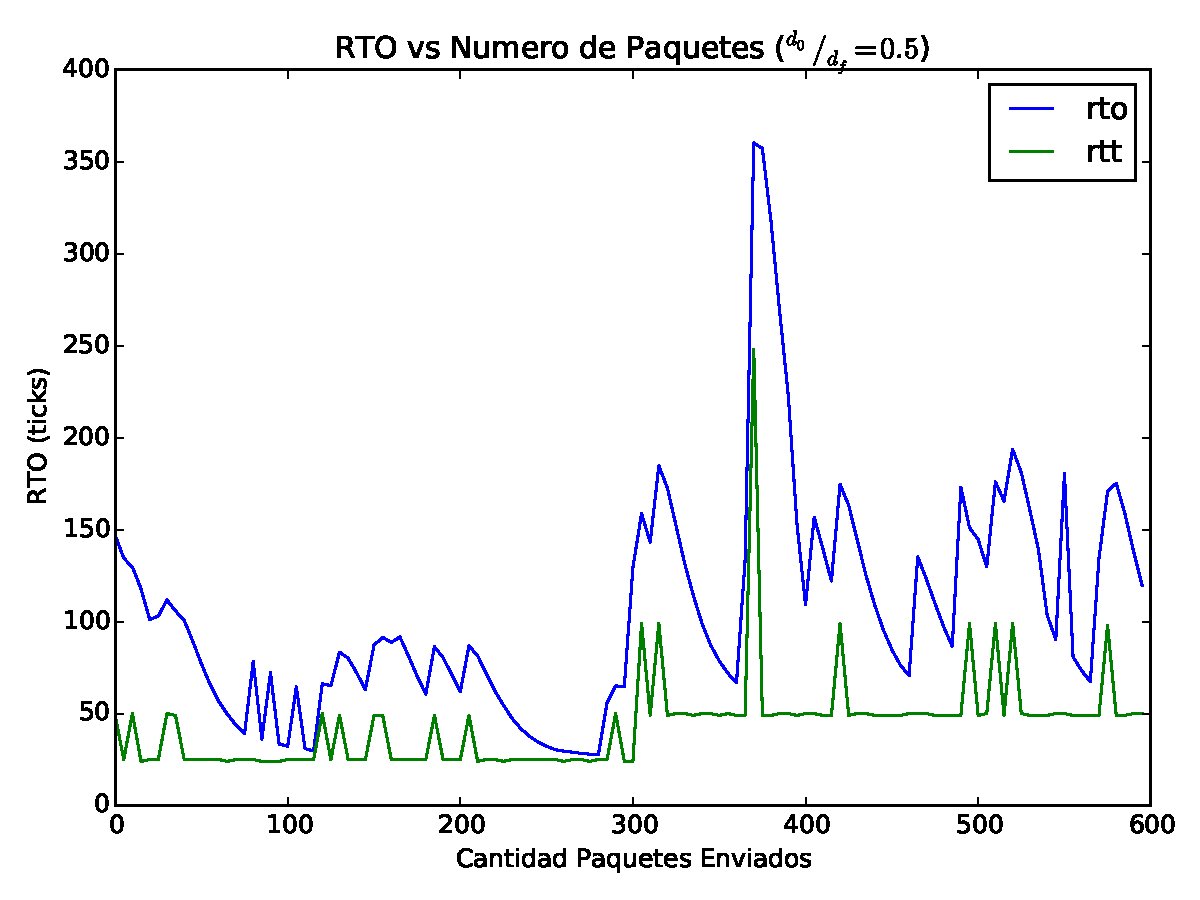
\includegraphics[width=0.32\textwidth]{imagenes/congestion_2.pdf}
		    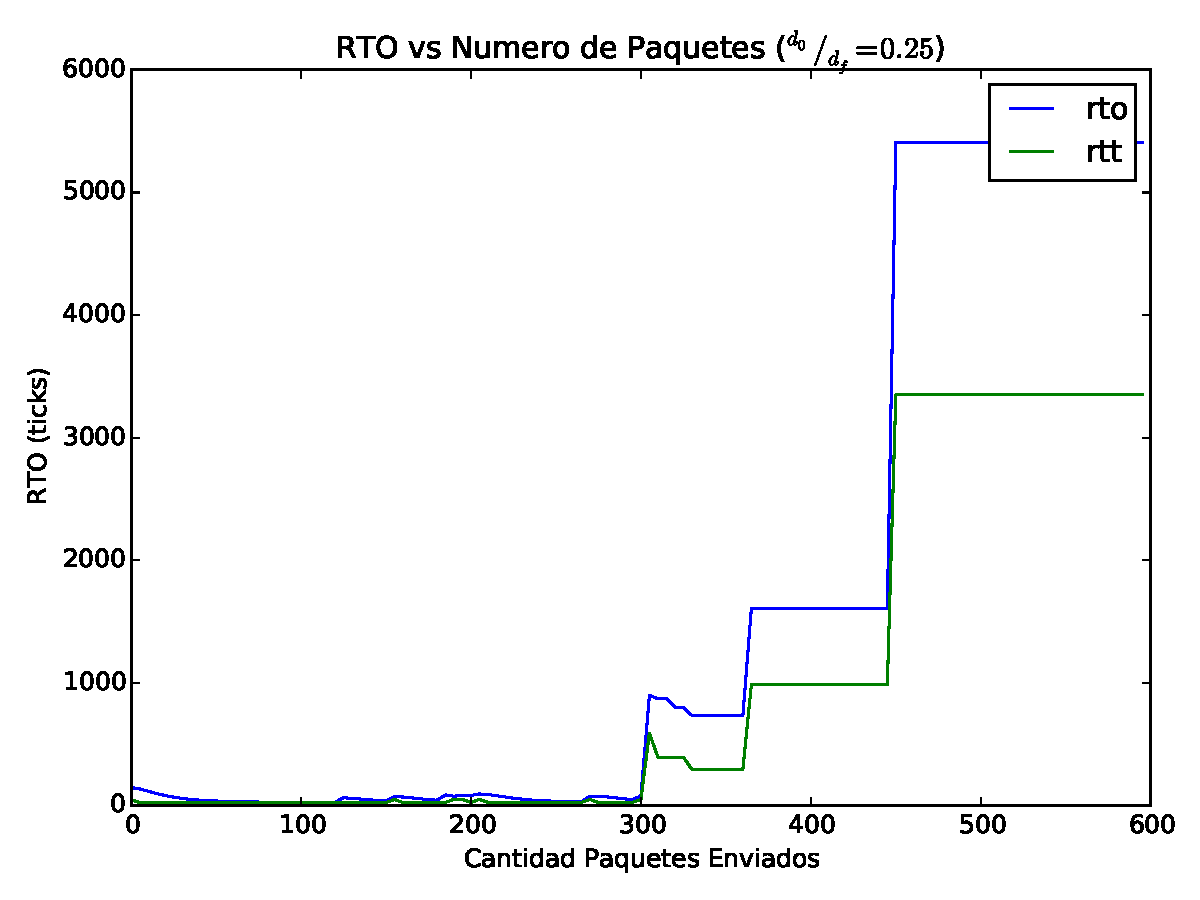
\includegraphics[width=0.32\textwidth]{imagenes/congestion_4.pdf}

            \caption*{Escenario 1}

        \end{figure}

		Como se puede ver, mientras en el primer caso con delay constante el RTO
		sube cuando hay un timeout, pero este mismo baja r\'apidamente y vuelve
		a un valor cercano al RTT bastante r\'apido.

		Cuando el timeout se duplica, el RTO tiene picos cuando hay un timeout,
		que son cada vez m\'as grandes y m\'as seguidos, pero al bajar nunca
		llega al RTT original. Esto se debe a que el cliente detecta que hay
		tanta ``congesti\'on'' que el protocolo intenta bajarla subiendo el
		tiempo hasta la pr\'oxima transmisi\'on, pero como esta nunca baja esta
		no se acerca tanto al RTT como en el primer caso.

		En el tercer caso, cuando el timeout se cuadruplica, la ``congesti\'on''
		parece ser tan grande que el RTO en el protocolo deja de tener un valor
		previsible ya que nunca llegan a un nivel estable con la cantidad de
		paquetes mandados.

        El \emph{Escenario 2} muestra el resultado en una red con
        par\'aemtros: $\alpha={{1}\over{8}}$, $\beta={{1}\over{2}}$
        cuando no se congestiona, cuando la congesti\'on causa el doble de
        delay, y cuando causa el cu\'adruple.

        \begin{figure}[H]
            \center

		    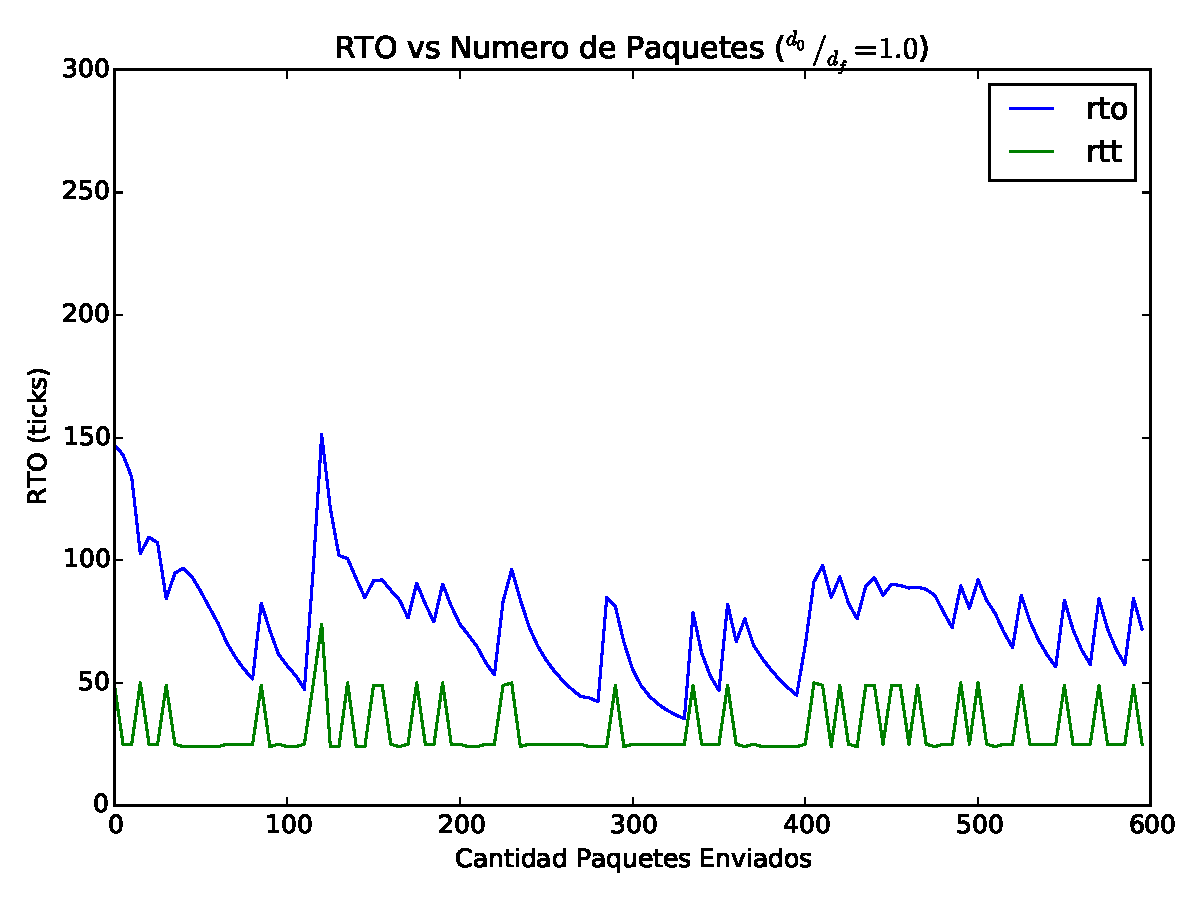
\includegraphics[width=0.32\textwidth]{imagenes/congestionb_1.pdf}
		    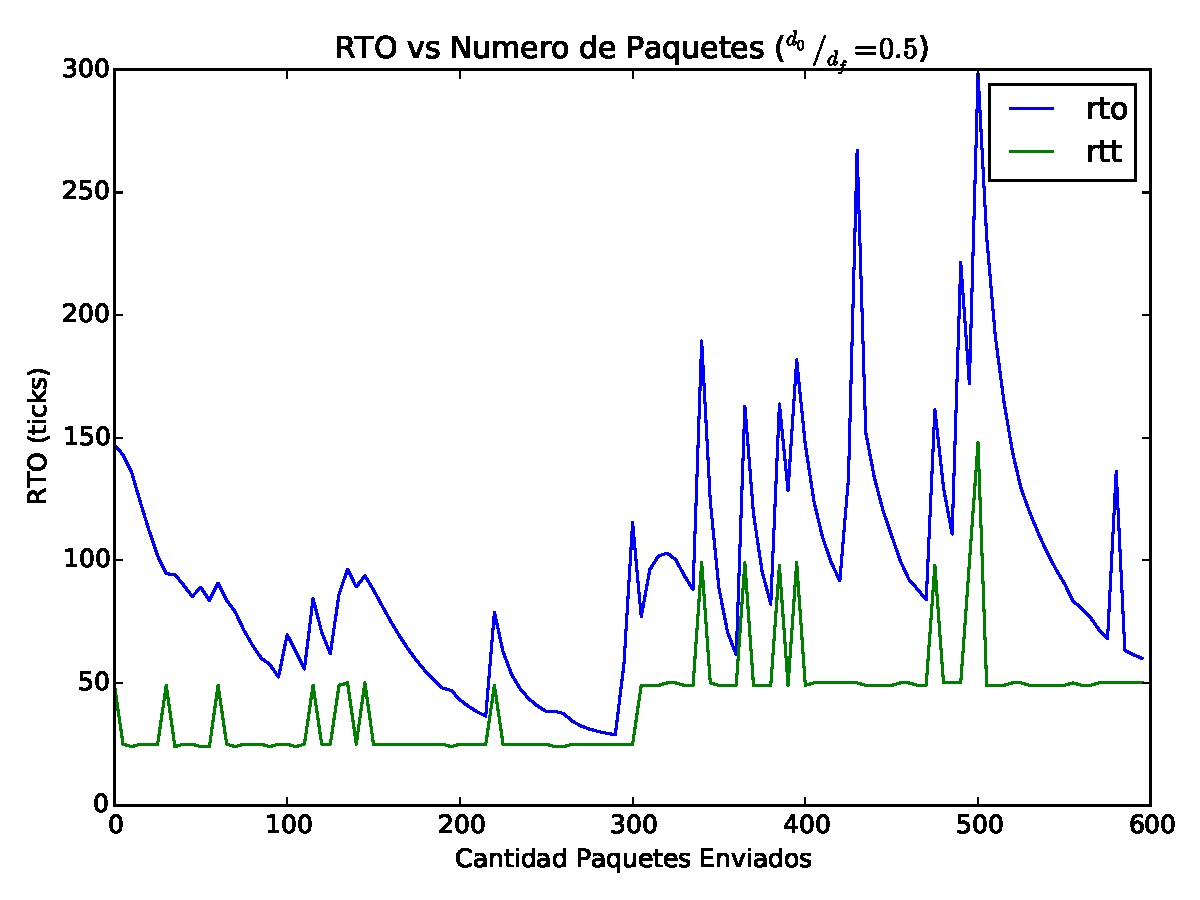
\includegraphics[width=0.32\textwidth]{imagenes/congestionb_2.pdf}
		    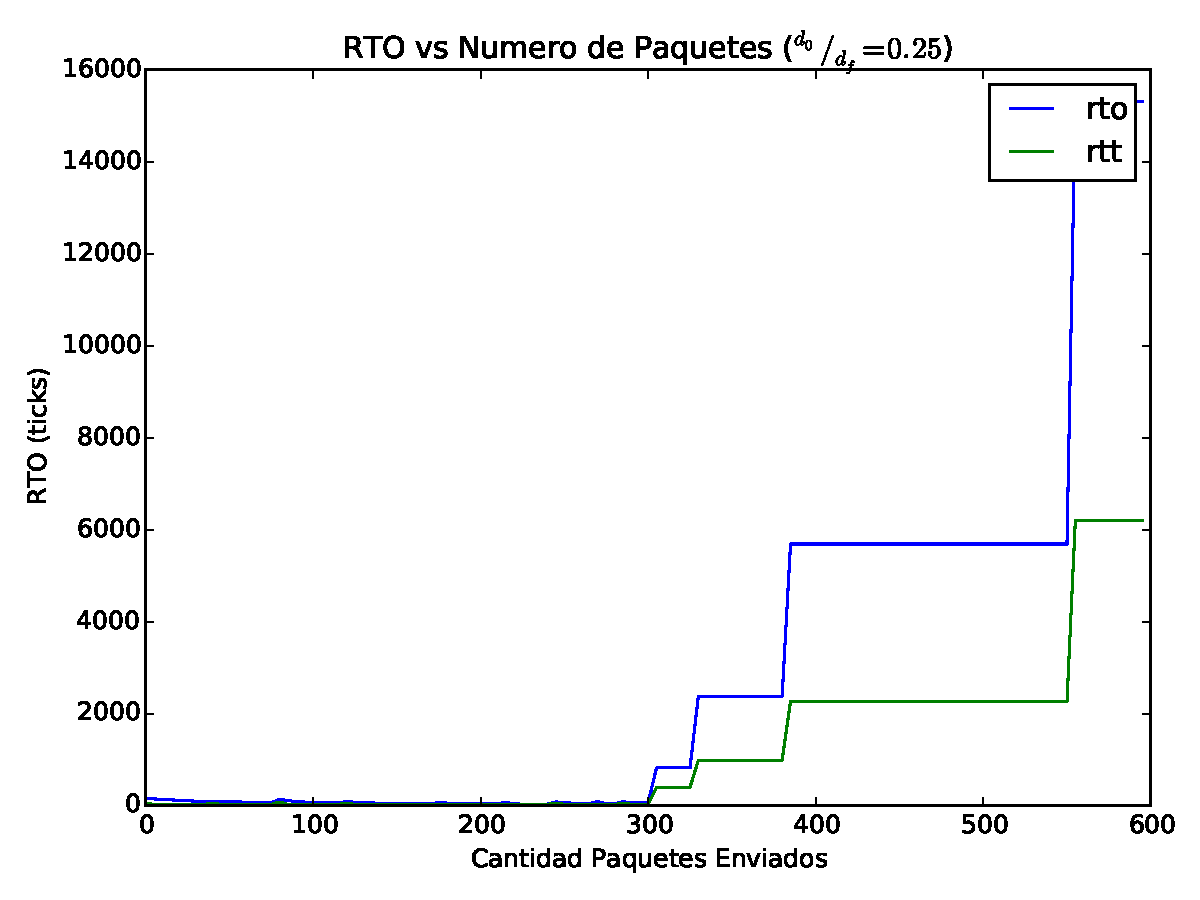
\includegraphics[width=0.32\textwidth]{imagenes/congestionb_4.pdf}

            \caption*{Escenario 2}

        \end{figure}

		En este caso sucede algo similar al caso del \emph{Escenario 1},
		sugiriendo que este resultado no depende en gran medida de los
		parametros $\alpha$ y $\beta$.

		\hspace{1em}

		Por \'ultimo, se intenta hacer un escenario largo donde el delay se
		duplica y se hace la mitad cada 300 paquetes, simulando una red donde
		el nivel de congesti\'on cambia bastante seguido. Esto se est\'a
		haciendo en una red con $\alpha = {{1}\over{2}}$ y $\beta =
		{{1}\over{4}}$.

		En este primer gr\'afico, tomamos sesiones con grupos de 500 paquetes,
		donde el delay de cada grupo es el doble o la mitad de el del grupo
		anterior.

		\begin{figure}[H]
			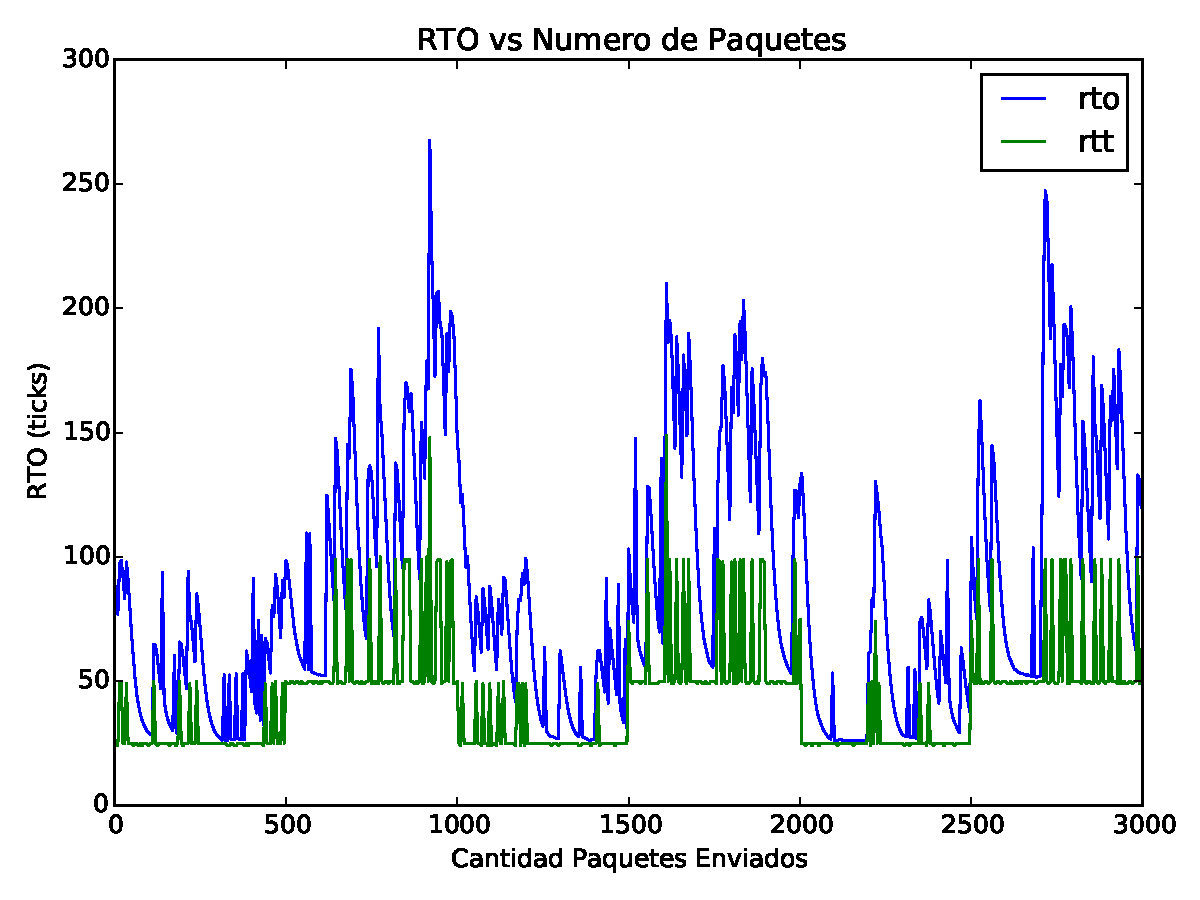
\includegraphics[width=\textwidth]{imagenes/congestion_long.pdf}
            \caption*{Escenario 3: grupos de 500 paquetes con delay 25, 50, 25, \ldots}
		\end{figure}


		Como podemos ver, el RTO promedio sube y tiene picos m\'as alejados del
		RTT cuando hay tanta congesti\'on que el delay se duplica, pero puede
		volver a la normalidad r\'apidamente cuando la congesti\'on para. Por
		otro lado, como podemos ver en la pr\'oxima figura, donde los grupos son
		de 100 paquetes

		\begin{figure}[H]
			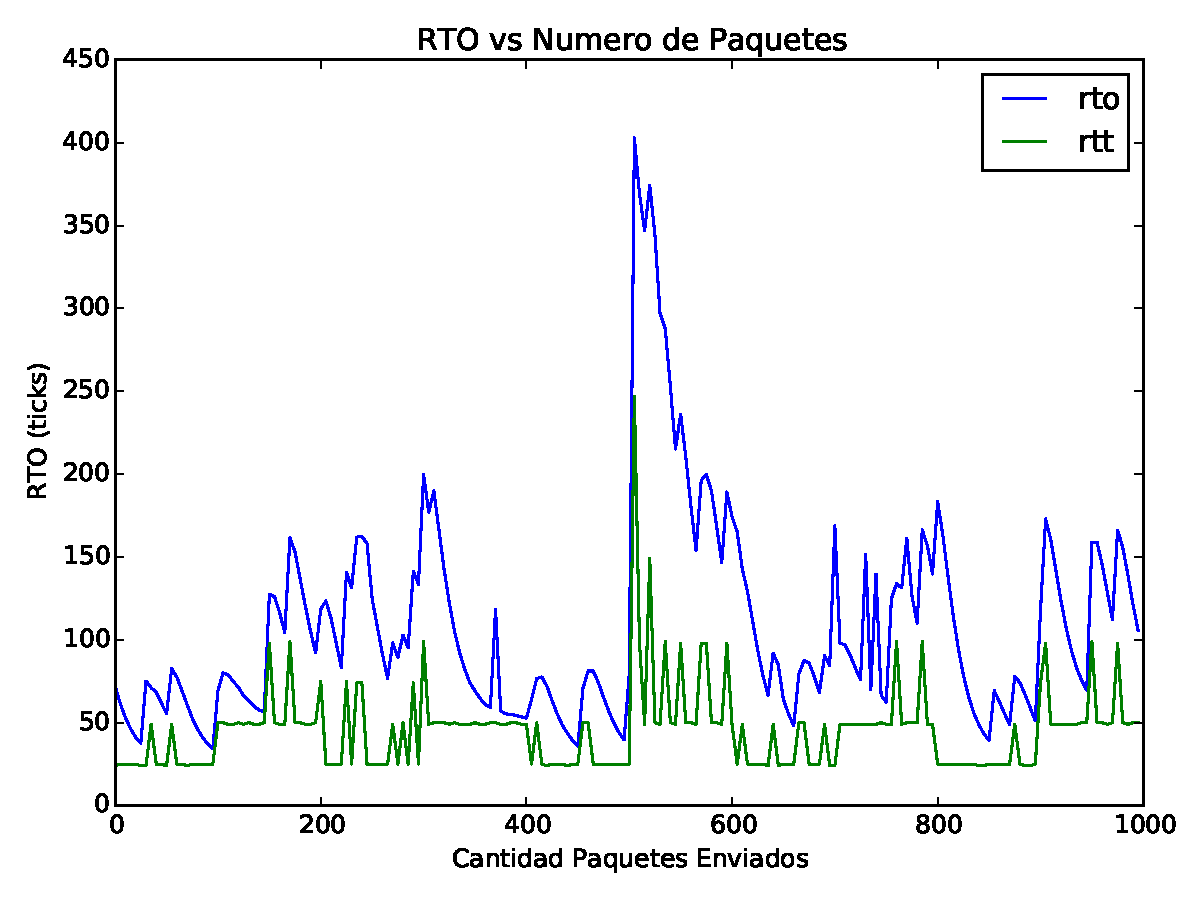
\includegraphics[width=\textwidth]{imagenes/congestion_short.pdf}
			\caption*{Escenario 4: grupos de 100 paquetes con delay 25, 50, 25, \ldots}
		\end{figure}

		Si los problemas de congesti\'on cambian cada menos paquetes, puede ser
		que el RTO no tenga tiempo para recuperrase y volver a valores m\'as
		cercanos al RTT.

    \subsection{Tiempo total de transmisi\'on en entorno con p\'erdidas}

        Para este experimento se configur\'o un escenario en el cual el
        cliente env\'ia 300 mensajes al servidor, pasados los 150 el delay
        se incrementa de \textit{25 ticks} a \textit{50 ticks}. A su vez,
        la probabilidad de perder un paquete es de 0.1.
        Luego, utilizando wireshark, se calcul\'o el tiempo que dur\'o la
        conexi\'on en base a los paquetes capturados y su timestamp.

        Para los valores de $\alpha=0$ y $\beta=0$ el tiempo fue 42,19 seg,
        para los valores propuestos por el RFC el tiempo promedio fue
        41,67 seg, para $\alpha=0.15$ y $\beta=0.2$ 42,39 seg, finalmente
        para $\alpha=1$ y $\beta=1$ el tiempo fue 44,34 seg.


